\documentclass[../../../../main.tex]{subfiles}
\begin{document}

\begin{flushright}
\footnotesize\textit{【自動文字起こし・要確認】}
\end{flushright}

[解] 点$X$に対し $\overrightarrow{OX} = \vec{x}$とすると
$\vec{a}, \vec{b}, \vec{c}$ は1次独立であり $\cdots \text{①}$
\begin{align*}
\vec{p_1} &= k\vec{a} \\
\vec{p_2} &= l\vec{a} + (1-l)\vec{b} \\
\vec{p_3} &= (1-m)\vec{b} + m\vec{c} \\
\vec{p_4} &= n\vec{c}
\end{align*}

(1) $\overrightarrow{P_1P_2} = \overrightarrow{P_4P_3}$ だから
\[ (l-k)\vec{a} + (1-l)\vec{b} = (1-m)\vec{b} + (m-n)\vec{c} \]
①から
\[ l-k=0, \quad m-n=0, \quad 1-l=1-m \]
\[ \therefore k = l = m = n \quad \text{(答)} \]

(2) (1)から $k = l = m = n \equiv \alpha$ とおく。
対角線の交点は、$P_1P_3$の中点だから、この点$X$として
\[ \vec{x} = \frac{1}{2} \left( \alpha\vec{a} + (1-\alpha)\vec{b} + \alpha\vec{c} \right) \cdots \text{②} \]
一方、$OB, AC$の中点$Y, Z$とすると
\[ \vec{y} = \frac{1}{2}\vec{b}, \quad \vec{z} = \frac{1}{2}(\vec{a}+\vec{c}) \]
だから、線分$YZ$上の点$W$は
\[ \vec{w} = \frac{1}{2} \{t(\vec{a}+\vec{c}) + (1-t)\vec{b}\} \quad (0 \le t \le 1) \]
の形でかける。$t = \alpha$ とすると ($0 < \alpha < 1$) ②から $\vec{w} = \vec{x}$ となるから、
題意は示された。(証明終)

\begin{center}
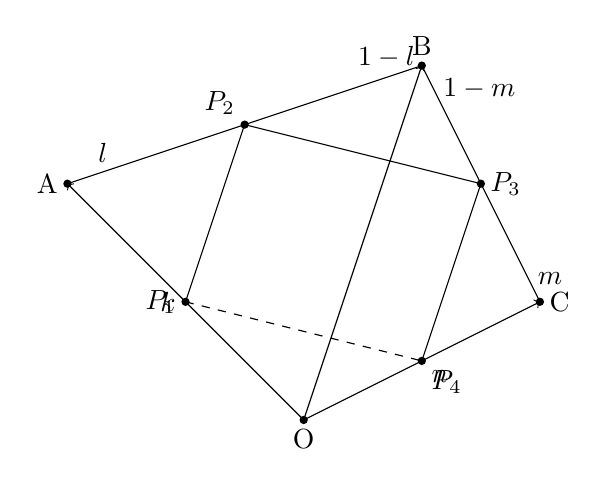
\begin{tikzpicture}[scale=1.5]
\coordinate (O) at (0,0);
\coordinate (A) at (-2,2);
\coordinate (B) at (1,3);
\coordinate (C) at (2,1);

\coordinate (P1) at (-1,1);
\coordinate (P2) at (-0.5,2.5);
\coordinate (P3) at (1.5,2);
\coordinate (P4) at (1,0.5);

\draw[->] (O) -- (A) node[midway, left] {$k$};
\draw[->] (O) -- (B);
\draw[->] (O) -- (C) node[midway, below right] {$n$};

\draw (A) -- (B) node[pos=0.1, above] {$l$} node[pos=0.9, above] {$1-l$};
\draw (B) -- (C) node[pos=0.1, right] {$1-m$} node[pos=0.9, right] {$m$};

\fill (O) circle (1pt) node[below] {O};
\fill (A) circle (1pt) node[left] {A};
\fill (B) circle (1pt) node[above] {B};
\fill (C) circle (1pt) node[right] {C};

\fill (P1) circle (1pt) node[left] {$P_1$};
\fill (P2) circle (1pt) node[above left] {$P_2$};
\fill (P3) circle (1pt) node[right] {$P_3$};
\fill (P4) circle (1pt) node[below right] {$P_4$};

\draw (P1) -- (P2) -- (P3) -- (P4);
\draw[dashed] (P1) -- (P4);
\end{tikzpicture}
\end{center}

\end{document}
